% LaTeX source for ``การเรียนรู้ของเครื่องสำหรับเคมีควอนตัม (Machine Learning for Quantum Chemistry)''
% Copyright (c) 2022 รังสิมันต์ เกษแก้ว (Rangsiman Ketkaew).

% License: Creative Commons Attribution-NonCommercial-NoDerivatives 4.0 International (CC BY-NC-ND 4.0)
% https://creativecommons.org/licenses/by-nc-nd/4.0/

\chapter{การเรียนรู้เชิงลึก}
\label{ch:dl}

เอาล่ะครับ ในบทนี้เราจะมาดูหัวข้อการเรียนรู้เชิงลึกหรือ Deep Learning ซึ่งเป็นหนึ่งใน Buzzword\footnote{สิ่งที่กำลังเป็นที่พูดถึงหรือได้รับความนิยม
โดยที่ฟังแล้วก็อาจจะเป็นคำเก๋ ๆ} ที่หลาย ๆ คนต่างก็พูดถึงในช่วงระยะเวลา 10 ปีที่ผ่านมา โดยเฉพาะอย่างยิ่งในระหว่างที่ผู้เขียนกำลังเขียนหนังสือเล่มนี้ 
ไม่ว่าจะเป็นวงการอาชีพไหน ๆ ก็จะต้องมีการนำ Deep Learning ไปใช้ทั้งนั้น และแน่นอนว่าหนึ่งในนั้นก็คือการนำมาประยุกต์ใช้ในงานวิจัยทางด้านเคมี 
ซึ่งข้อมูลที่นักเคมีมีอยู่ในมือนั้นมากมายมหาศาล ดังนั้นจึงน่าสนใจว่า Deep Learning จะช่วยนักเคมีในการขับเคลื่อนงานวิจัยได้อย่างไร

\begin{figure}[H]
    \centering
    \includegraphics[width=0.7\linewidth]{fig/wisard.png}
    \caption{เครื่องการเรียนรู้เชิงลึก WISARD เครื่องแรกของโลก ณ พิพิธภัณฑ์วิทยาศาสตร์ กรุงลอนดอน ประเทศอังกฤษ 
    (เครดิตภาพ: รังสิมันต์ เกษแก้ว)}
    \label{fig:wisard}
\end{figure}

จริง ๆ แล้ว Deep Learning นั้นถือว่าเป็นโครงข่ายประสาทเทียม (Neural Network) ซึ่งเป็นเทคนิคปัญญาประดิษฐ์แบบหนึ่งที่ถูกพัฒนาขึ้นมาเพื่อศึกษา%
รูปแบบที่แน่นอนของข้อมูลเรียกว่า การรับรู้รูปแบบ (Pattern Recognition) ซึ่งเป็นกระบวนที่ทำงานเลียนแบบ (Mimic) สมองของมนุษย์ในการแยก%
แยะความจำเพาะเจาะจงบางอย่างออกมาจากข้อมูลที่ป้อนเข้าไป ภาพที่ \ref{fig:wisard} แสดงเครื่อง WISARD ซึ่งเป็นคอมพิวเตอร์เครื่องแรกของ%
โลกที่ถูกสร้างขึ้นมาในปี ค.ศ. 1981 สำหรับการคำนวณ Deep Learning

ในบทก่อนหน้านี้นั้นเราได้พูดถึง Supervised Learning กันไปแล้ว ซึ่งจะเป็นการทำนายค่า $y$ จากข้อมูลนำเข้า $x$ โดยเป็นการพิจารณาในกรณี%
ของการถดถอยเชิงเส้น ในลำดับถัดมา (ซึ่งก็คือในบทนี้) เราจะมาพิจารณากรณีที่พารามิเตอร์ของเรานั้นมีความไม่เป็นเชิงเส้น (Nonlinear) กันครับ
ซึ่งโมเดลปัญญาประดิษฐ์ที่ถูกนำมาใช้อย่างแพร่หลายนั้นก็คือ Neural Network นั่นเอง โดยเฉพาะ Deep Learning ที่ ณ ปัจจุบันได้มีการพัฒนาและ%
ปรับปรุงจนมีประสิทธิภาพที่สูงมาก

%--------------------------
\section{การเรียนรู้ของโมเดลที่ไม่เป็นเชิงเส้น}
\label{sec:nonlinear_ml}
\idxboth{การเรียนรู้ของโมเดลที่ไม่เป็นเชิงเส้น}{Nonlinear Supervised Learning}
%--------------------------

สมมติว่าเรามี $\{(x^{(i)}, y^{(i)})\}^n_{i=1}$ ซึ่งเป็นตัวอย่างชุดข้อมูลฝึกสอน (Training Data) และเราจะเริ่มกันด้วยกรณีที่ง่ายที่สุด%
นั่นก็คือ $y^{(i)} \in \mathbb{R}$ และ $h_\theta(x) \in \mathbb{R}$ 

เราจะทำการกำหนด Cost/Loss Function ขึ้นมา ซึ่งเราจะใช้ Least Square Cost function สำหรับข้อมูลลำดับที่ $i$ นั่นก็คือคู่อันดับ 
$(x^{(i)} ,y^{(i)} )$ ดังนี้ 

\begin{equation}\label{eq:loss}
    J^{(i)} (\theta) = \frac{1}{2} \left(h_\theta (x^{(i)}) - y^{(i)}\right)^2
\end{equation}

\noindent และกำหนด Mean-Square Cost Function สำหรับชุดข้อมูลดังนี้

\begin{equation}\label{eq:mse_loss}
    J(\theta) = \frac 1 n \sum_{i=1}^n J^{(i)}(\theta)
\end{equation}

\noindent ซึ่งผู้อ่านอาจจะสังเกตได้ว่าสมการข้างต้นนั้นจะเหมือนกับในกรณีของ Linear Regression เว้นแต่จะต่างกันตรงที่เราได้มีการเพิ่ม $1/n$
เข้าไปในด้านหน้าของ Cost Function \footnote{การคูณ Cost Function ด้วยปริมาณสเกลาร์ เช่น ตัวเลข จะไม่ทำให้จุดต่ำสุดสัทพันธ์ 
(Local minima) และจุดต่ำสุดสัมบูรณ์ (Global Minima) เปลี่ยนไป} นอกจากนี้ผู้อ่านจะต้องทำความเข้าใจด้วยว่าการปรับค่าพารามิเตอร์ 
(Parameterization) ของ $h_\theta(x)$ นั้นจะแตกต่างจากกรณีของ Linear Regression ถึงแม้ว่าเราจะใช้ Cost Function ที่เหมือน%
กันก็ตาม 

ลำดับถัดมาคือตัวปรับค่าพารามิเตอร์ (Optimizer) ซึ่งโดยทั่วไปแล้วเรามักจะใช้ Stochastic Gradient Descent (SGD) นั่นก็เพราะว่าเป็นวิธีที่%
ง่ายและไม่ซับซ้อนสำหรับการปรับค่าให้เหมาะสม (Optimize) Loss Function ของเราซึ่งเขียนแทนด้วย $J(\theta)$ ซึ่งการปรับค่านั้นจะใช้%
สมการดังต่อไปนี้\footnote{สังเกตว่าเราใช้เครื่องหมาย $a := b$ เพื่อบ่งบอกการดำเนินการ (Operation) ซึ่งเป็นการระบุค่าให้กับตัวแปรใน%
โปรแกรมคอมพิวเตอร์}

\begin{equation}
    \theta := \theta - \alpha\nabla_\theta J(\theta)
\end{equation}

\noindent โดยที่ $\alpha$ คืออัตราเร็วในการเรียนรู้ \textit{Learning Rate} หรืออาจจะเรียกว่า \textit{Step Size} ก็ได้ 
โดยเรามักจะกำหนดให้ค่า $\alpha$ มีค่ามากกว่าศูนย์ ด้านล่างคืออัลกอริทึมของ SGD

\begin{algorithm}[ht]
    \caption{อัลกอริทึมของ Stochastic Gradient Descent}
    \label{alg:sgd_dl}
    \begin{algorithmic}
    \State Hyperparameter: learning rate $\alpha$, number of total iteration $n_\text{iter}$.
    \State Initialize $\theta$ randomly.
    \For{$i = 1$ to $n_\text{iter}$}
        \State Sample $j$ uniformly from ${1,\ldots,n}$, and update $\theta$ by
        \begin{equation*}
            \theta := \theta - \alpha\nabla_\theta J^{(j)}(\theta)
        \end{equation*}
    \EndFor
    \end{algorithmic}
\end{algorithm}

ในทางปฏิบัตินั้นการคำนวณ Gradient ของ $B$ หลาย ๆ ครั้งสามารถทำพร้อมกันได้เพราะว่าในปัจจุบันเรามีเทคนิคการทำการคำนวณแบบขนาน 
(Parallelization) สำหรับการปรับค่า $\theta$ ซึ่งจะเร็วกว่าการคำนวณ Gradient ของ $B$ แบบแยกกันทีละค่าแน่นอน ซึ่งการที่เราจะทำ%
การคำนวณแบบพร้อม ๆ กันได้นั้นเราจะต้องมีการแบ่ง Data ของเราออกเป็นส่วนย่อย ๆ แล้วทำการคำนวณแยกกัน (Batch) ซึ่งเราจะต้องมีการปรับ%
อัลกอริทึมเล็กน้อย โดยด้านล่างคืออัลกอริทึมของ Mini-batch SGD ซึ่งได้จากการปรับอัลกอริทึมของ SGD แบบธรรมดา  

\begin{algorithm}[ht]
    \caption{อัลกอริทึมของ Mini-batch Stochastic Gradient Descent}
    \label{alg:sgd_minibatch}
    \begin{algorithmic}
    \State Hyperparameter: learning rate $\alpha$, batch size $B$, \# iteration $n_\text{iter}$.
    \State Initialize $\theta$ randomly.
    \For{$i = 1$ to $n_\text{iter}$}
        \State Sample $j$ uniformly from ${1,\ldots,n}$, and update $\theta$ by
        \State Sample $B$ examples $j_1,\ldots,j_B$ (without replacement) uniformly from $\{1,\ldots,n\}$, 
        and update $\theta$ by
        \begin{equation*}
            \theta := \theta - \frac{\alpha}{B}\sum_{k=1}^B\nabla_\theta J^{(j_k)}(\theta)
        \end{equation*}
    \EndFor
    \end{algorithmic}
\end{algorithm}

โดยทั่วไปแล้วโมเดล Deep Learning นั้นจะมีการเรียนรู้ซึ่งอาศัยอัลกอริทึมตามด้านบนโดยทำตามขั้นตอนดังต่อไปนี้

\begin{enumerate}
    \item กำหนด $h_\theta(x)$
    \item เขียนอัลกอริทึม Backpropagation เพื่อคำนวณ Gradient ของ Loss Function $J^{(j)}(\theta)$
    \item ทำการปรับ Loss Function โดยใช้ SGD หรือ Mini-batch SGD หรือใช้ Optimizer ตัวอื่น ๆ
\end{enumerate}

%--------------------------
\section{โครงข่ายประสาทเทียม}
\label{sec:nn}
\idxboth{โครงข่ายประสาทเทียม}{Neural Network}
%--------------------------

โครงข่ายประสาทเทียม (Neural Network)

การเรียนรู้เชิงลึกรูปแบบที่มาตรฐานที่สุดคือการเรียนรู้แบบมีผู้สอนด้วยโมเดลแบบไม่เป็นเชิงเส้น (Supervised learning with nonlinear model)

%--------------------------
\section{การแผร่กระจายการเรียนรู้}
\idxboth{การแผร่กระจายการเรียนรู้}{Learning Propagation}
%--------------------------

การแผร่กระจายการเรียนรู้ (Learning Propagation) เป็นขั้นตอนการเรียนรู้ของโมเดล Neural Network ที่เลียนแบบการทำงานของสมอง 


\begin{figure}[H]
\begin{center}
    \begin{tikzpicture}[x=2.2cm,y=1.4cm]
    \message{^^JNeural network with arrows}
    \readlist\Nnod{4,5,5,5,3} % array of number of nodes per layer
    
    \message{^^J  Layer}
    \foreachitem \N \in \Nnod{ % loop over layers
    \edef\lay{\Ncnt} % alias of index of current layer
    \message{\lay,}
    \pgfmathsetmacro\prev{int(\Ncnt-1)} % number of previous layer
    \foreach \i [evaluate={\y=\N/2-\i; \x=\lay; \n=\nstyle;}] in {1,...,\N}{ % loop over nodes
    
    % NODES
    \node[node \n] (N\lay-\i) at (\x,\y) {$a_\i^{(\prev)}$};
    %\node[circle,inner sep=2] (N\lay-\i') at (\x-0.15,\y) {}; % shifted node
    %\draw[node] (N\lay-\i) circle (\R);
    
    % CONNECTIONS
    \ifnum\lay>1 % connect to previous layer
    \foreach \j in {1,...,\Nnod[\prev]}{ % loop over nodes in previous layer
    \draw[connect arrow] (N\prev-\j) -- (N\lay-\i); % connect arrows directly
    %\draw[connect arrow] (N\prev-\j) -- (N\lay-\i'); % connect arrows to shifted node
    }
    \fi % else: nothing to connect first layer
    
    }
    
    }
    
    % LABELS
    \node[above=5,align=center,mygreen!60!black] at (N1-1.90) {input\\[-0.2em]layer};
    \node[above=2,align=center,myblue!60!black] at (N3-1.90) {hidden layers};
    \node[above=8,align=center,myred!60!black] at (N\Nnodlen-1.90) {output\\[-0.2em]layer};
    
    \end{tikzpicture}
    \caption{โครงข่ายประสาทแบบสมบูรณ์ (Dense Neural Network)}
\end{center}
\end{figure}

จะเห็นได้ว่าไดอะแกรมด้านบนนั้นมีความซับซ้อนมาก ซึ่งจริง ๆ แล้วถ้าหากเราจะมาทำความเข้าใจองค์ประกอบของ Neural Network นั้น เราควร%
พิจารณากรณีง่าย ๆ ด้วยโครงสร้างแบบเล็ก ๆ ก่อน ตามภาพที่ \ref{fig:nn_layer} ซึ่งเป็นชั้นการเรียนรู้ (Learning Layer) ประกอบไปด้วย
3 ส่วน ดังนี้

\begin{description}
    \item[Input Layer] ชั้นอินพุต เก็บข้อมูลที่เราจะนำมาใช้ในการฝึกสอนโมเดล โดยในแต่ละหน่วยประสาท (Neuron) จะเป็นตัวที่เก็บคุณลักษณ์%
    ที่อยู่ในข้อมูล เช่น ความยาวพันธะ จำนวนเวเลนซ์อิเล็กตรอนของอะตอม
    \item[Hidden Layer] ชั้นที่ถูกซ่อนไว้ เป็นชั้นที่อยู่ระหว่างชั้นอินพุตและชั้นเอาต์พุต โดยข้อมูลที่ถูกส่งมาจากชั้นก่อนหน้า (ในที่นี้คือชั้นอินพุต)
    จะถูกนำไปผ่านฟังก์ชันกระตุ้น (Activation Function) ในชั้นนี้ และหลังจากนั้นจะถูกส่งออกไปชั้นต่อไป (ในที่นี้คือชั้นเอาต์พุต)
    \item[Output Layer] ชั้นเอาต์พุต เป็นชั้นสุดท้ายของโครงข่ายประสาท โดยจะรับข้อมูลหรืออินพุตมาจากชั้นก่อนหน้าซึ่งเป็น Hidden Layer
    โดยในชั้นนี้อาจจะมีการนำฟังก์ชันกระตุ้นมาใช้หรือไม่ใช้ก็ได้
\end{description}

\begin{figure}[H]
    \centering
    \subfloat[ชั้นการเรียนรู้ (Learning Layer)\label{fig:nn_layer}]{
        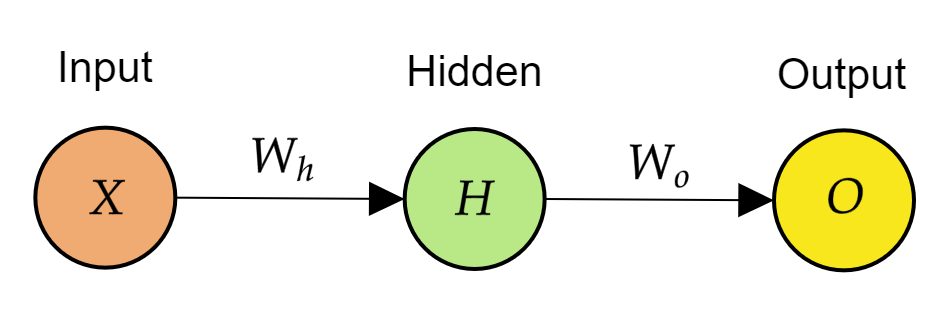
\includegraphics[width=0.45\linewidth]{fig/nn_layer.png}}
    \hspace{1em}
    \subfloat[โครงข่ายแบบค่าน้ำหนักหลายตัว\label{fig:nn_w_matrices}]{
        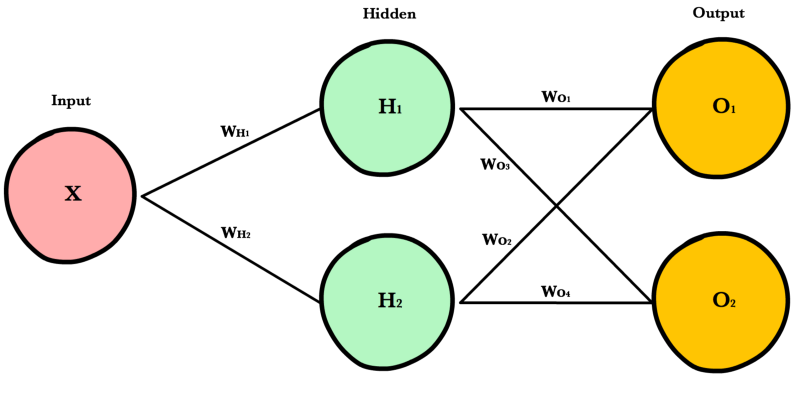
\includegraphics[width=0.45\linewidth]{fig/nn_w_matrices.png}}
    \caption{ตัวอย่างของโครงข่ายประสาทแบบง่าย}
    \label{fig:nn_layer_w}
\end{figure}

โดยเราสามารถใช้โค้ดต่อไปนี้ในการสร้าง Neural Network แบบง่าย ๆ ได้

\begin{lstlisting}[style=MyPython]
def relu(z):
    return max(0,z)

def feed_forward(x, Wh, Wo):
    # Hidden layer
    Zh = x * Wh
    H = relu(Zh)

    # Output layer
    Zo = H * Wo
    output = relu(Zo)
    return output
\end{lstlisting}

เมื่อเราพิจารณาภาพที่ \ref{fig:nn_w_matrices} ซึ่งมีความซับซ้อนมากขึ้นโดยมีการเพิ่มจำนวน Neuron เข้าไปในชั้น Hidden Layer และ 
Output Layer เราจะพบว่าค่าน้ำหนักที่ถูกคำนวณออกมาจากชั้น Input จะถูกส่งไปยังชั้น Hidden และค่าน้ำหนักที่ออกมาจากชั้น Hidden ก็ถูก%
ส่งต่อไปยังชั้น Output ตามลำดับ โดยจะเห็นว่าทุก ๆ Neuron ของชั้นที่ถูกติดกันนั้นจะมีการแลกเปลี่ยนกันทุก Neuron โดยสมการที่ใช้ในการคำนวณ%
หาเอาต์พุตของแต่ละ Neuron มีดังนี้

\noindent $\bullet$ อินพุต 1 ตัว
\begin{align}\label{eq:nn_one_input}
    Z &= Input \cdot Weight \nonumber \\
    &= X W
\end{align}

\noindent $\bullet$ อินพุตมากกว่า 1 ตัว
\begin{align}\label{eq:nn_multi_input}
    Z &= \sum_{i=1}^{n}x_i w_i \nonumber \\
    &= x_1 w_1 + x_2 w_2 + x_3 w_3
\end{align}

เราจะสังเกตได้ว่าสมการที่ \ref{eq:nn_one_input} และ \ref{eq:nn_multi_input} เป็นสมการที่เหมือนกับที่เราใช้ใน Linear 
Regression เป๊ะ ๆ เลย ซึ่งจริง ๆ แล้ว Neural Network ที่มีจำนวน Neuron แค่ 1 อันนั้นคือ Linear Regression เลย แต่สิ่งที่ต่างกันก็คือ
Neural Network จะมีกระบวนที่เกี่ยวข้องกับค่าน้ำหนักและฟังก์ชันกระตุ้นด้วย สำหรับการกำหนดค่าน้ำหนักในช่วงเริ่มต้นของการฝึกสอนนั้นเราสามารถ%
กำหนดค่าได้โดยใช้การสุ่มค่าตามตัวอย่างโค้ดดังต่อไปนี้

\begin{lstlisting}[style=MyPython]
INPUT_LAYER = 1
HIDDEN_LAYER = 2
OUTPUT_LAYER = 2

def init_weights():
    Wh = np.random.randn(INPUT_LAYER, HIDDEN_LAYER) \
            * np.sqrt(2.0/INPUT_LAYER)
    Wo = np.random.randn(HIDDEN_LAYER, OUTPUT_LAYER) \
            * np.sqrt(2.0/HIDDEN_LAYER)
\end{lstlisting}

\noindent และเรามักจะกำหนดค่าเริ่มต้นของความโน้มเอียง (Bias) ด้วยค่าน้อย ๆ เช่น 0.1 หรือ 0.2 ดังตัวอย่างต่อไปนี้

\begin{lstlisting}[style=MyPython]
def init_bias():
    Bh = np.full((1, HIDDEN_LAYER), 0.1)
    Bo = np.full((1, OUTPUT_LAYER), 0.1)
    return Bh, Bo
\end{lstlisting}

%--------------------------
\subsection{การแผ่กระจายแบบไปข้างหน้า}
\label{sec:forward_prop}
\idxboth{การแผร่กระจายการเรียนรู้!การแผ่กระจายแบบไปข้างหน้า}{Propagation!Forward Propagation}
%--------------------------

ในขั้นเริ่มต้นของการฝึกสอนโมเดล Neural Network นั้น โมเดลจะยังไม่มีพารามิเตอร์ที่ถูกต้อง ดังนั้นเราจึงต้องสุ่มค่าเริ่มต้นของพารามิเตอร์ขึ้นมาก่อน
หลังจากนั้นจึงทำ Forward Propagation รอบที่หนึ่งแล้วก็เปรียบเทียบผลการทำนายกับคำตอบ (Output) ที่โมเดลทราบก่อนหน้านั้นแล้ว
ขั้นตอนต่อมาคือการปรับพารามิเตอร์ที่สำคัญอีกสองตัวนั่นคือน้ำหนัก (Weight) และความอคติหรือความโน้มเอียง (Bias) ให้มีค่าที่ถูกต้อง ซึ่งใน%
ขั้นตอนนี้เราจะใช้กระบวนการที่ตรงข้ามกันเรียกว่า Backward propagation โดยการทำ Propagation ทั้งสองแบบพร้อม ๆ กันครบหนึ่งรอบนั้น%
จะเรียกว่า 1 Epoch แต่ต้องระวังนะครับว่า Epoch, Batch Size และ Iteration นั้นมีความหมายต่างกัน โดยความแตกตางมีดังนี้

\begin{description}[font=$\bullet$~\normalfont\scshape\bfseries\color{red!50!black}]
    \item[1 Epoch] การทำ Forward และ Backward Propagation 1 ครั้ง
    \item[Batch Size] จำนวนของข้อมูลที่ใช้ในการฝึกสอนในการทำ Forward และ Backward Propagation 1 รอบ
    \item[Iteration] จำนวนของรอบในการฝึกสอน ซึ่งแต่ละรอบจะใช้ Batch Size ที่ถูกกำหนดไว้ก่อนการฝึกสอน
\end{description}

เพื่อให้เห็นภาพมากขึ้น เราลองมาดูตัวอย่างกัน เช่น ถ้าเรามีจำนวนข้อมูลในการฝึกสอน 1000 ตัวอย่างและกำหนด Batch Size เป็น 500 จะได้ว่าโมเดลของเรา%
จะใช้ 2 Iterations สำหรับการฝึกสอน 1 Epoch

\begin{figure}[H]
    \centering
    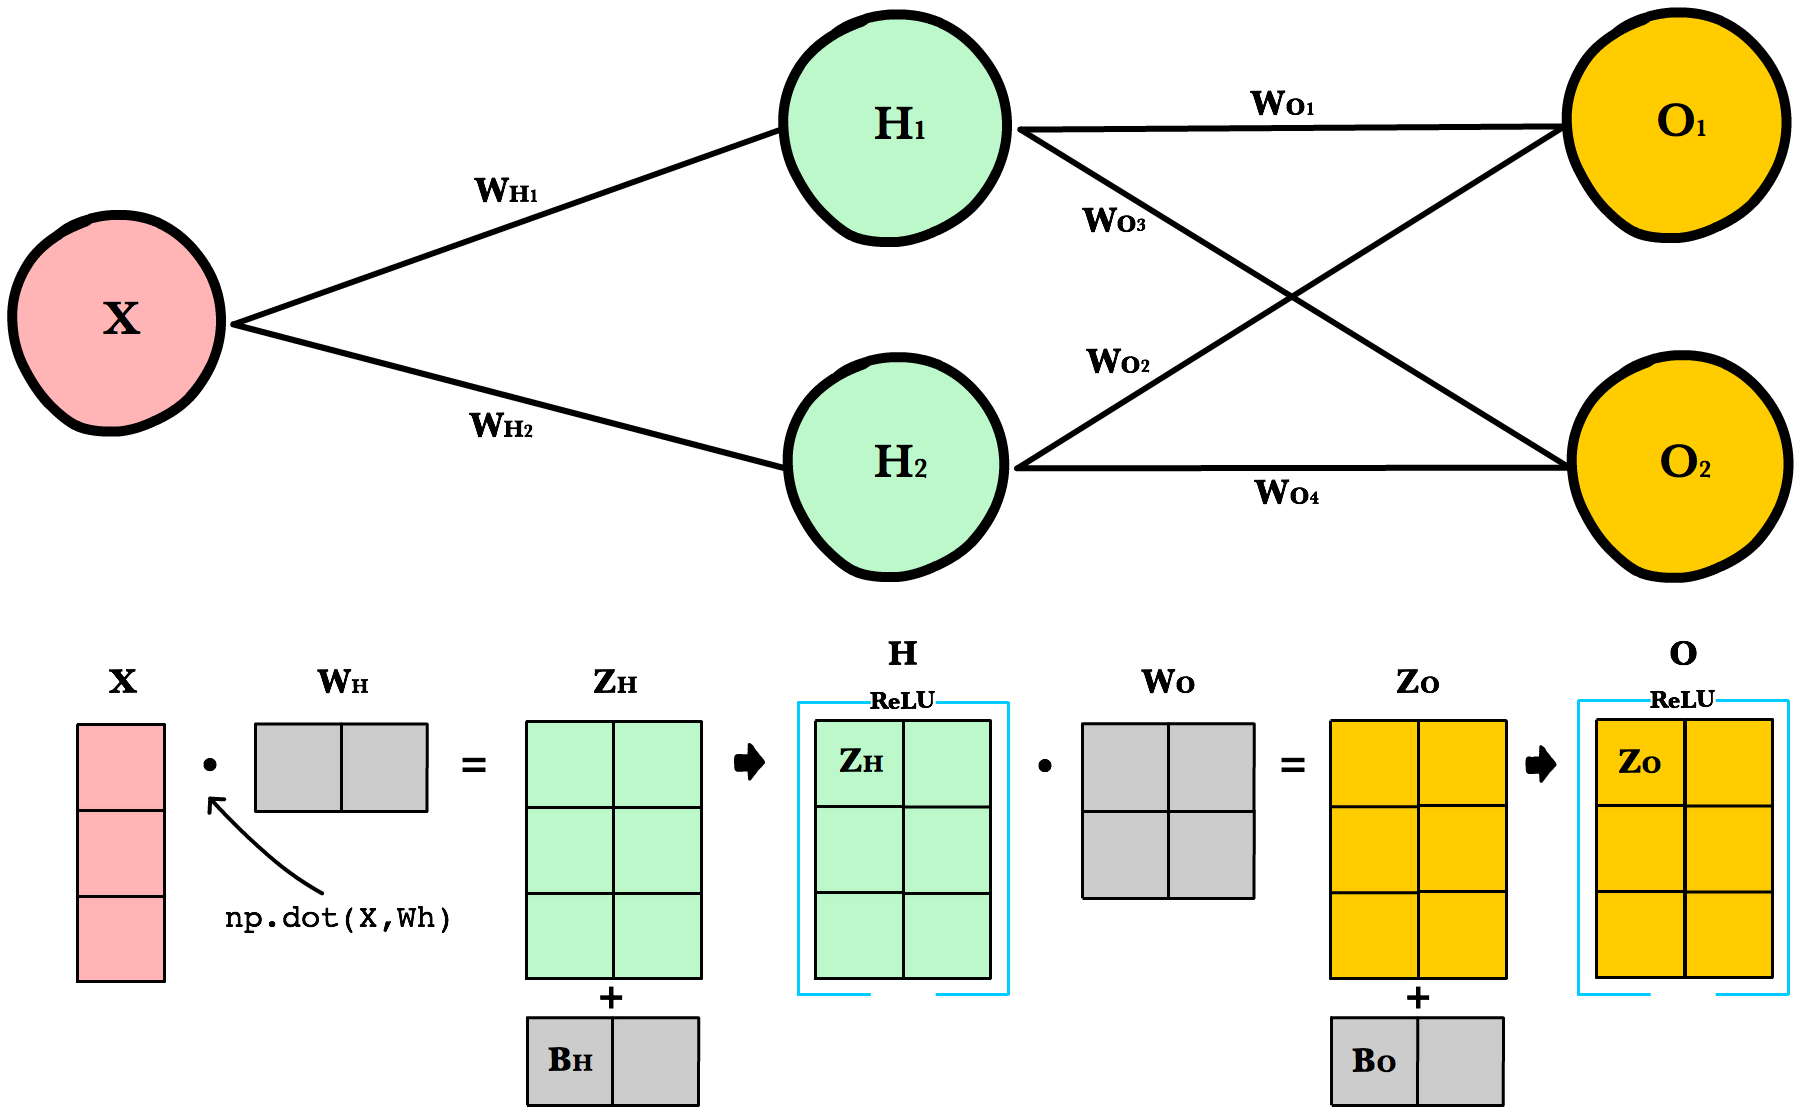
\includegraphics[width=0.9\linewidth]{fig/nn_feedforward_matrices.png}
    \caption{แผนภาพการดำเนินการคูณเมทริกซ์อินพุนด้วยเมทริกซ์น้ำหนัก}
    \label{fig:nn_ff_mat}
\end{figure}

\begin{figure}[H]
    \centering
    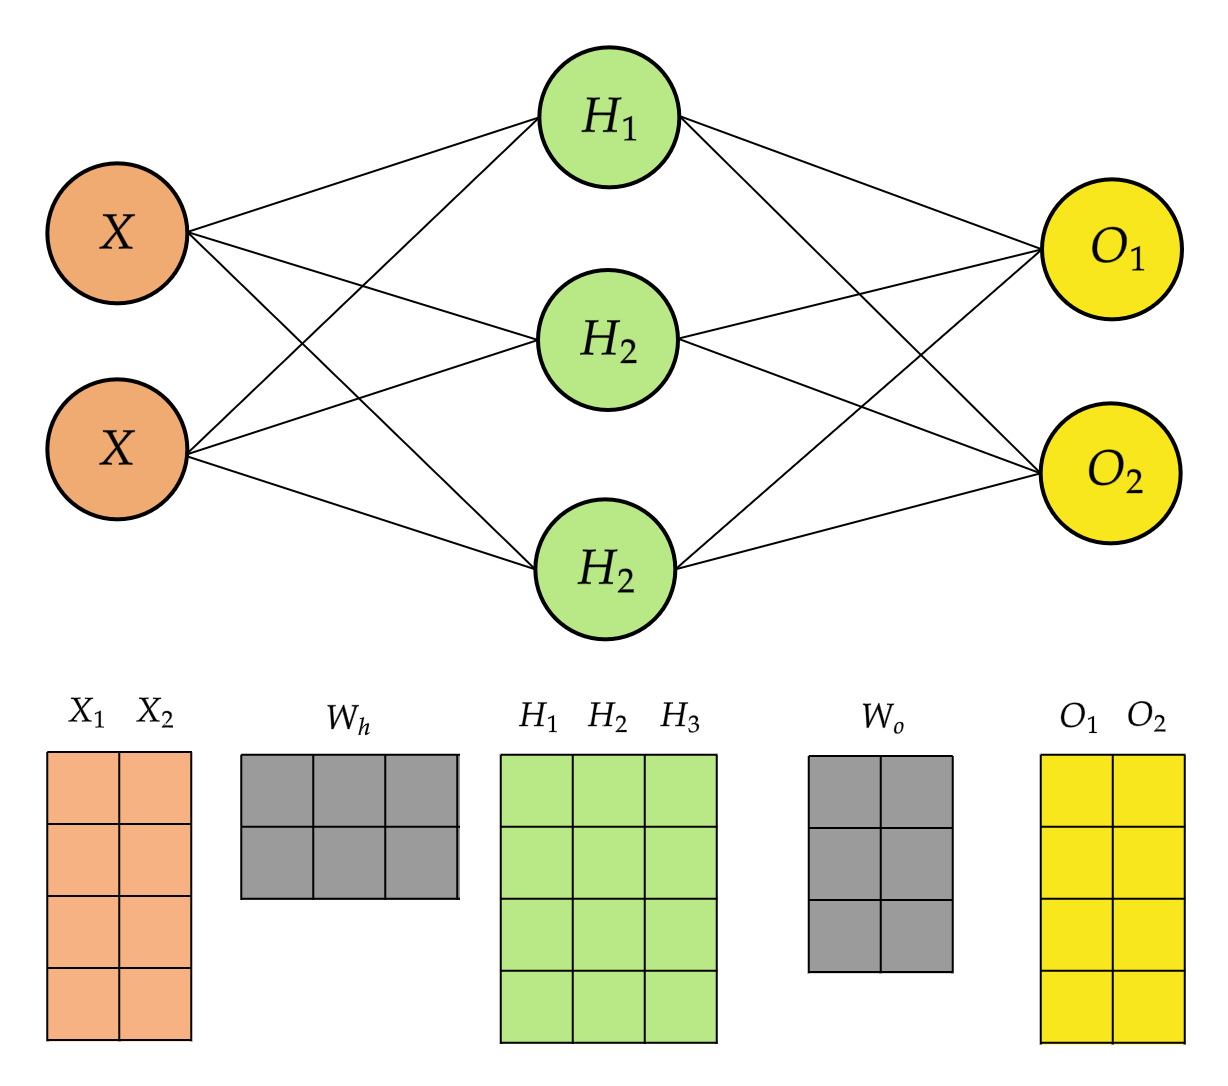
\includegraphics[width=0.8\linewidth]{fig/nn_feedforward_dyn_resizing.png}
    \caption{แผนภาพขนาดของเมทริกซ์ที่สามารถปรับขนาดได้แบบไดนามิกส์}
    \label{fig:nn_ff_dyn_resize}
\end{figure}

\begin{figure}[H]
    \centering
    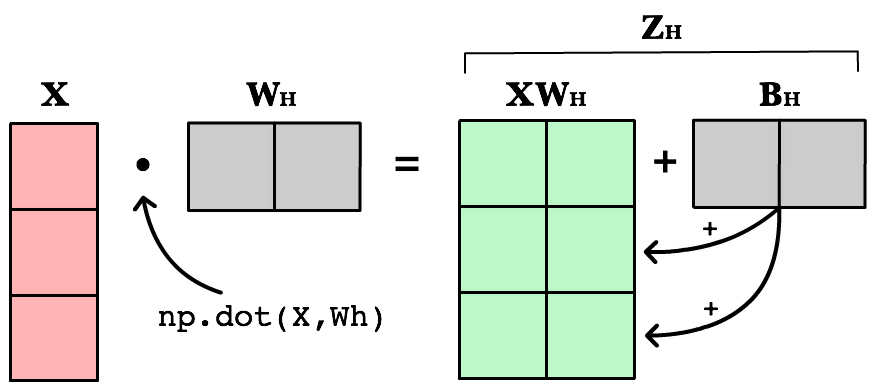
\includegraphics[width=0.8\linewidth]{fig/nn_feedforward_matrix_weighted_input.png}
    \caption{แผนภาพการดำเนินการคูณเมทริกซ์น้ำหนักและการเพิ่มความโน้มเอียง}
    \label{fig:nn_ff_mat_w}
\end{figure}

%--------------------------
\subsection{การแผ่กระจายแบบย้อนกลับ}
\label{sec:backprop}
\idxboth{การแผร่กระจายการเรียนรู้!การแผ่กระจายแบบย้อนกลับ}{Propagation!Backpropagation}
%--------------------------

การแผ่กระจายแบบย้อนกลับ (Backpropagation)

\begin{figure}[H]
    \centering
    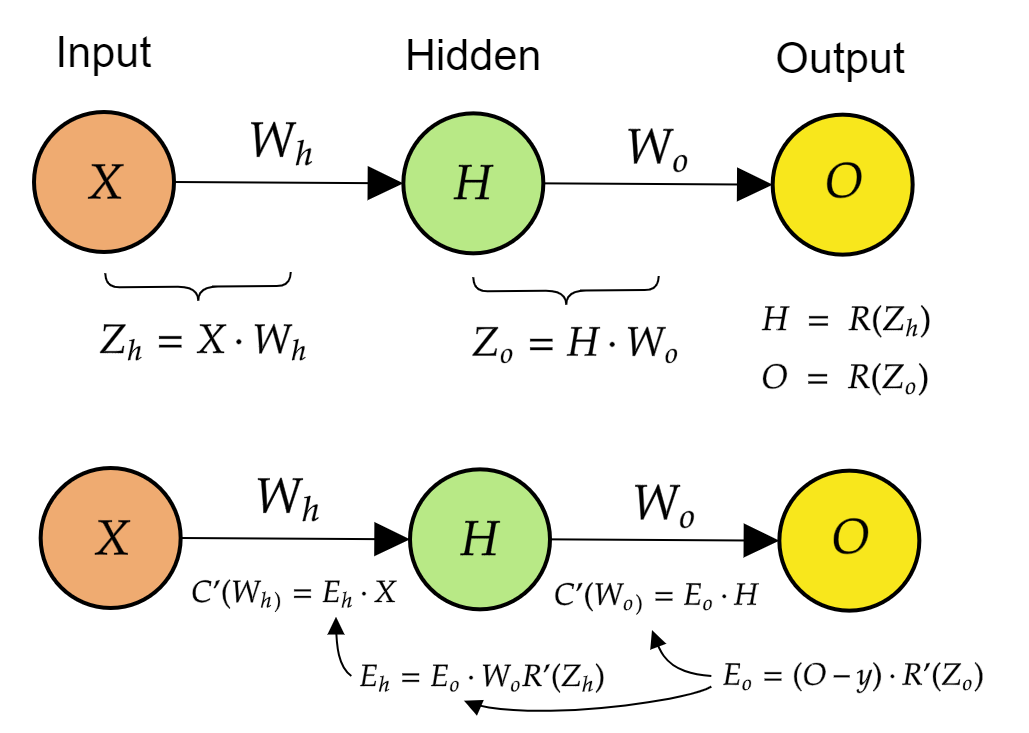
\includegraphics[width=0.8\linewidth]{fig/nn_backprop.png}
    \caption{การคำนวณการแผ่กระจายแบบย้อนกลับจากชั้นเอาต์พุตไปยังชั้นอินพุน}
    \label{fig:nn_bp}
\end{figure}

%--------------------------
\section{ฟังก์ชันกระตุ้น}
\label{sec:act_func}
\idxboth{ฟังก์ชันกระตุ้น}{Activation Function}
%--------------------------

ฟังก์ชันกระตุ้น (Activation Function)

\begin{itemize}
    \item Linear
    \begin{figure}[H]
        \centering
        \subfloat[%
        \begin{equation}
            \begin{split}R(z,m) = \begin{Bmatrix} z*m \\
            \end{Bmatrix}\end{split}
        \end{equation}
        ]{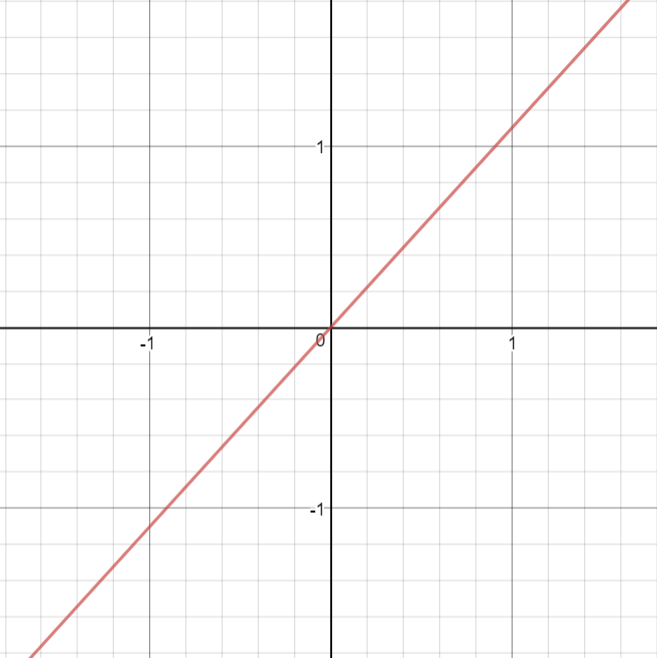
\includegraphics[width=0.4\linewidth]{fig/actfunc_linear.png}}
        \hspace{1em}
        \subfloat[%
        \begin{equation}
            \begin{split}R'(z,m) = \begin{Bmatrix} m \\
            \end{Bmatrix}\end{split}
        \end{equation}
        ]{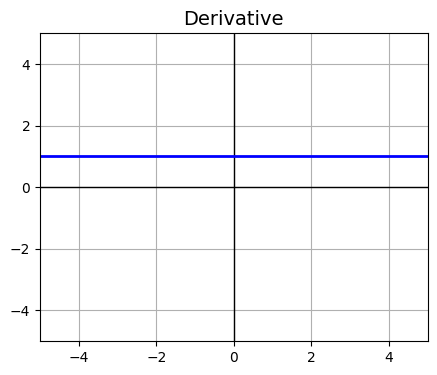
\includegraphics[width=0.4\linewidth]{fig/actfunc_linear_der.png}}
    \end{figure}
    \item ELU
    \item ReLU
    \item LeakyReLU
    \item Sigmoid
    \item Tanh
    \item Softmax
    \begin{equation}
        \sigma(z_i) = \frac{e^{z_{i}}}{\sum_{j=1}^K e^{z_{j}}} \ \ \ for\ i=1,2,\dots,K
    \end{equation}
\end{itemize}

%--------------------------
\section{ฟังก์ชันความคลาดเคลื่อน}
\label{sec:loss_func}
\idxboth{ฟังก์ชันความคลาดเคลื่อน}{Loss Function}
%--------------------------

ฟังก์ชันความคลาดเคลื่อน (Loss Function หรือ Cost Function หรือ Error Function) สำหรับโจทย์ประเภท Regression ของชุดข้อมูล%
ที่มี $n$ จำนวนข้อมูล และมีค่าที่ได้จากการทำนายที่เป็น $\hat{y}$ และคำตอบ (Label) คือ $y$ มีดังต่อไปนี้

\begin{equation}\label{eq:mae}
    \text{MAE} = \frac{1}{n} \sum_{i=1}^{n} | y_{i} - \hat{y}_{i} |
\end{equation}

\begin{equation}\label{eq:mape}
    \text{MAPE} = \frac{1}{n} \sum_{i=1}^{n} \left| \frac{y_{i} - \hat{y}_{i}}{x_{i}} \right| \times 100
\end{equation}

\begin{equation}\label{eq:mse}
    \text{MSE} = \frac{1}{n} \sum_{i=1}^{n} \left( y_{i} - \hat{y}_{i} \right)^2
\end{equation}

\begin{equation}\label{eq:maxae}
    \text{MaxAE} = max\{y_{i} - \hat{y}_{i}\}, i = 1, 2, ..., n
\end{equation}

\begin{equation}\label{eq:maxape}
    \text{MaxAPE} = max\left\{\left| \frac{y_{i} - \hat{y}_{i}}{x_{i}} \right| \times 100 \right\}, i = 1, 2, ..., n
\end{equation}

\begin{equation}\label{eq:rmsd}
    \text{RMSD} = \sqrt{ \frac{1}{n} \sum_{i=1}^{n} (y_{i} - \hat{y}_{i})^{2} }
\end{equation}

\begin{equation}\label{eq:grmsd}
    \text{GRMSD} = \sqrt[2n]{ \prod_{i=1}^{n} (y_{i} - \hat{y}_{i})^{2} }
\end{equation}

\begin{equation}\label{eq:gwrmsd}
    \text{GWRMSD} = \sqrt{ \frac{\sum_{i=1}^{n} \zeta_{i} (y_{i} - \hat{y}_{i})^{2}}{\sum_{i=1}^{n} \zeta_{i} } }
\end{equation}

\noindent โดยที่ $\zeta_{i} = e^{-(y_{i} - \hat{y}_{i}) / c}$

\begin{equation}\label{eq:huber}
    L_{\delta}=
    \left\{\begin{matrix}
        \frac{1}{2}(y - \hat{y})^{2} & \text{if} \left | (y - \hat{y})  \right | < \delta\\
        \delta ((y - \hat{y}) - \frac1 2 \delta) & \text{otherwise}
    \end{matrix}\right.
\end{equation}

สำหรับ Loss Function ที่ \ref{eq:mae} - \ref{eq:gwrmsd} จะมีความคล้ายคลึงกัน แต่จะต่างกันตรงที่การปรับรูปแบบให้ฟังก์ชันที่เป็นความ%
แตกต่างระหว่างค่าอ้างอิงและค่าทำนายนั้นมีความไว (Sensitivity) ต่อ Outlier ที่ต่างกันไป สำหรับสมการที่ \ref{eq:huber} นั้นคือ Huber
Loss ซึ่งจะมีความไวต่อค่าที่ห่างค่าผิดปกติ (Outlier)\footnote{ค่าผิดปกติหรือ Outlier คือค่าที่อยู่ห่างจากค่าส่วนใหญ่ในชุดข้อมูลมากเกินไป} 
ที่น้อยกว่ากรณีของ MSE (สมการที่ \ref{eq:mse}) เพราะว่าใน MSE เทอม $y_{i} - \hat{y}_{i}$ ถูกกำลังสองอยู่นั่นเอง

ฟังก์ชันความคลาดเคลื่อนสำหรับโจทย์ประเภท Classification

\noindent $\bullet$ Cross-entropy คือการวัดความแตกต่างระหว่างการกระจายตัวของความน่าจะเป็น 2 กลุ่มของตัวแปรแบบสุ่มของเหตุการณ์%
ที่เราสนใจ (กลุ่มหรือ Class ในชุดข้อมูล) โดยกรณีที่มีแค่ 2 Class $(M = 2)$ เราจะเรียกประเภทนี้ว่า Binary Cross-entropy และกรณีที่%
มีมากกว่า 2 Class ($M > 2$) เราจะเรียกว่า Multiclass Cross-entropy ซึ่งทั้งสองแบบมีสมการดังต่อไปนี้

\begin{equation}
    H(p) = -{(y\log(p) + (1 - y)\log(1 - p))}
\end{equation}

\begin{equation}
    H(p) = -\sum_{c=1}^My_{o,c}\log(p_{o,c})
\end{equation}


\noindent โดยที่ $p$ คือความน่าจะเป็นของการสังเกต $o$ ใน Class $c$ และ $y$ คือตัวระบุ Class (เช่น 0 กับ 1)

\noindent $\bullet$ Negative Log-likelihood (NLL)

\begin{equation}
    l(y) = -{\log(p(y))}
\end{equation}

\noindent $\bullet$ Hinge loss

\begin{equation}
    l(y) = max(0, 1 - y \cdot \hat{y})
\end{equation}

\noindent $\bullet$ Kullback-Leibler (KL) Divergence

\begin{equation}
    KL(\hat{y} || y) = \sum_{c=1}^{M}\hat{y}_c \log \bigg( {\frac{\hat{y}_c}{y_c}} \bigg)
\end{equation}

\noindent $\bullet$ Jensen-Shannon (JS) Divergence

\begin{equation}
    JS(\hat{y} || y) = \frac{1}{2}(KL(y||\frac{y+\hat{y}}{2}) + KL(\hat{y}||\frac{y+\hat{y}}{2}))
\end{equation}

%--------------------------
\section{ตัวประเมินโมเดล}
\label{sec:metrics}
\idxboth{ตัวประเมินโมเดล}{Metrics}
%--------------------------

สิ่งที่เราใช้ในการประเมินหรือวัดประสิทธิภาพของโมเดลก็คือ Metrics ซึ่ง Metrics สำหรับโจทย์ประเภท Regression นั้นเราสามารถใช้ฟังก์ชัน%
ที่เป็น Loss Function ได้เลย แต่กรณีโจทย์ประเภท Classification นั้นเราจะต้องใช้ฟังก์ชันที่ต่างกันออกไป ฟังก์ชันต่อไปนี้คือ Metrics 
ที่มักจะถูกใช้เป็น Metrics สำหรับ Classification

\noindent $\bullet$ ประเภทวัดความถูกต้องและแม่นยำ

\begin{equation}
    \text{Accuracy} = \frac{TP+TN}{TP+TN+FP+FN}
\end{equation}

\begin{equation}
    \text{Precision} = \frac{TP}{TP+FP}
\end{equation}

\begin{equation}
    \text{Recall} = \frac{TP}{TP+FN}
\end{equation}

\begin{align}
    \text{F1} &= \frac{2*Precision*Recall}{Precision+Recall} \nonumber \\
    &= \frac{2*TP}{2*TP+FP+FN}
\end{align}

\noindent $\bullet$ ประเภทวัดความว่องไวและความจำเพาะเจาะจง

\begin{equation}
    \text{Sensitivity} = \text{Recall} = \frac{TP}{TP+FN}
\end{equation}

\begin{equation}
    \text{Sensitivity} = \frac{TN}{FP+TN}
\end{equation}

\noindent นอกจากนี้ยังมี Area Under the Curve (AUC) ซึ่งเป็นการใช้พื้นที่ใต้เส้นโค้งสำหรับการแบ่งกลุ่ม (Classifier) อีกด้วย

%--------------------------
\section{ตัวปรับความเหมาะสม}
\label{sec:optimizer}
\idxboth{ตัวปรับความเหมาะสม}{Optimizer}
%--------------------------

ตัวปรับความเหมาะสมหรือปรับประสิทธิภาพการเรียนรู้ของโมเดล (Optimizer) เป็นฟังก์ชันทางคณิตศาสตร์ซึ่งขึ้นอยู่กับพารามิเตอร์ที่เรียนรู้ได้ของโมเดล 
เช่น Weight และ Bias ซึ่ง Optimizer เป็นสิ่งที่จะช่วยให้โมเดลทราบวิธีการเปลี่ยน Weight และ Learning Rate ของ Neural Network 
เพื่อลดค่า Loss หรือ Error ที่เกิดขึ้นให้น้อยลงในแต่ละรอบของการฝึกสอนโมเดล

ตัวอย่างของ Optimizer ที่ได้รับความนิยมและมีประสิทธิภาพที่ยอดเยี่ยม

\noindent $\bullet$ Stochastic Gradient Descent (SGD) เป็นฟังก์ชันที่อัพเดทค่าพารามิเตอร์ในทุก ๆ ชุดข้อมูลที่ใช้ในการฝึกฝน SGD 
เป็นอัลกอริทึมที่ค่อนข้างไว โดยอัพเดทแค่ครั้งเดียวต่อการฝึกสอนโมเดล 1 รอบ นอกจากนี้ยังมีสิ่งที่เรียกว่าโมเมนตัม (Momentum) ซึ่งถูกพัฒนา%
ขึ้นมาเพื่อเร่งความเร็วในการ Opitmization ของ SGD โดยจะเป็นตัวที่เข้ามาแก้ปัญหาความแปรปรวนที่เกิดขึ้นใน SGD ซึ่งทำให้เกิดความยากในการ%
ที่จะลู่เข้าจุดที่ต่ำที่สุดได้ โดยการให้ความสำคัญในการพุ่งไปยังทิศทางที่ใกล้จุดกลางมากที่สุดก่อนแล้วทำให้ทิศทางที่ไม่เกี่ยวข้องความสำคัญลดลง

\noindent $\bullet$ Mini Batch Gradient Descent ถูกพัฒนาขึ้นเพื่อแก้ปัญหาของ Gradient Descent (GD) โดยการนำข้อดีของ GD 
แบบธรรมดาและ SGD มารวมกัน โดยสำหรับอัลกอริทึมนี้จะทำการอัพเดทค่าเป็น \enquote{ชุด} โดยภายในแต่ละชุดจะประกอบด้วยข้อมูลจำนวน 
$n$ ข้อมูล เราจึงเรียกเทคนิคนี้ว่าเป็น Mini Batch หรือจำนวนชุดข้อมูลขนาดเล็กนั่นเอง

\noindent $\bullet$ Adagrad เป็นฟังก์ชันที่สามารถปรับค่าอัตราเร็วในการเรียนรู้ (Learning Rate) ให้เหมาะสมกับพารามิเตอร์ได้ 
โดยจะมีการอัพเดทจำนวนมากสำหรับค่าพารามิเตอร์ที่มีจำนวนน้อย และอัพเดทน้อยถ้าค่าพารามิเตอร์มีจำนวนมากและด้วยเหตุนี้ Optimizer 
ตัวนี้จึงเป็นที่นิยมสำหรับข้อมูลที่มีการกระจายตัว (Sparse Data)

\noindent $\bullet$ Adadelta เป็นฟังก์ชันที่พัฒนาต่อจาก AdaGrad โดยสามารถแก้ปัญหา Decaying Learning Rate ที่เกิดขึ้นใน 
AdaGrad ได้ โดยเคล็ดลับก็คือแทนที่จะเก็บสะสมการคำนวณทั้งหมดที่ผ่านมาของ Gradient ใน AdaDelta นั้นจะถูกจำกัดการสะสมค่าการคำนวณของ 
Gradient ได้เองเพื่อแก้ขนาดค่าของน้ำหนักที่จะเกิดขึ้น หมายความว่าแทนที่เราจะเก็บค่าน้ำหนักที่ได้รับการอัพเดทมาก่อนหน้านี้ที่ยังไม่เวิร์ค 
เราจะเปลี่ยนเป็นการหาผลรวมของ Gradients แทน ซึ่งจะทำแบบนี้ซ้ำไปเรื่อย ๆ เพื่อการแก้ปัญหา Decaying Learning Rate ของ Gradients 
ที่ผ่านมาทั้งหมด

\noindent $\bullet$ Adam ย่อมาจาก \enquote{Adaptive Moment Estimation} เป็นวิธีการสุ่มเกรเดียนท์ที่อิงจากการประมาณค่าแบบปรับตัว 
(Adaptive Estimation) ของช่วงเวลาอันดับที่หนึ่งและอันดับสอง ซึ่งความสามารถของ Adam ก็คือสามารถปรับอัตราเร็วของการเรียนรู้พารามิเตอร์%
ในแต่ละครั้งได้และยังสามารถแก้ปัญหาการลดลงที่เร็วเกินไป (Decaying) ของ Gradients ในแต่ละ Step ที่ผ่านมาได้เหมือนกับ AdaDelta 
อีกทั้งยังอธิบายการเกิด Decaying Average ของ Gradients ที่ผ่านมาได้อีกด้วย ซึ่งจะเหมือนกับโมเมนตัมนั่นเอง

Adam เป็นอัลกอริทึมเป็นที่นิยมมากที่สุดเพราะรวมข้อดีของแต่ละอัลกอริทึมที่อธิบายไว้ก่อนหน้านี้เข้าด้วยกัน และแก้ปัญหาหรือข้อบกพร่อมออกไป 
เช่น Decaying Learning Rate ของ Adagrad และยังมีความเร็วที่มากกว่า GD และลดปัญหาการแกว่งของพารามิเตอร์ได้อีกด้วย

\noindent $\bullet$ Conjugate Gradients

\noindent $\bullet$ BFGS

\noindent $\bullet$ Momentum

\noindent $\bullet$ Nesterov Momentum

\noindent $\bullet$ Newton's Method

\noindent $\bullet$ RMSProp


ตัวอย่างโค้ดของการเรียกใช้ SGD Optimizer ของ TensorFlow

\begin{lstlisting}[style=MyPython]
# Create an optimizer with the desired parameters.
opt = tf.keras.optimizers.SGD(
    learning_rate=0.01,
    momentum=0.0,
    nesterov=False,
    name='SGD',
    **kwargs
)

# `loss` is a callable that takes no argument and returns the value
# to minimize.
loss = lambda: 3 * var1 * var1 + 2 * var2 * var2

# In graph mode, returns op that minimizes the loss by updating the listed
# variables.
opt_op = opt.minimize(loss, var_list=[var1, var2])
opt_op.run()

# In eager mode, simply call minimize to update the list of variables.
opt.minimize(loss, var_list=[var1, var2])
\end{lstlisting}

%--------------------------
\section{สถาปัตยกรรมของโครงข่ายประสาท}
\label{sec:architecture}
\idxboth{สถาปัตยกรรมของโครงข่ายประสาท}{Neural Network Architecture}
%--------------------------

สถาปัตยกรรมของโครงข่ายประสาทเทียม (Architecture)

%--------------------------
\section{ตัวอย่างการสร้างและฝึกสอนโมเดลด้วย TensorFlow}
%--------------------------

ในหัวข้อนี้จะเป็นการยกตัวอย่างประกอบโค้ดของการสร้างและฝึกสอนโมเดลในการทำนายค่าสภาพการละลายของโมเดล ซึ่งค่าสภาพการละลายหรือ
Solubility เป็นความสามารถของสสารในการละลายในน้ำ ยิ่งมีค่าเยอะหมายความว่าสสารนั้นยิ่งละลายในน้ำได้ดี โดยเราจะใช้ Module Keras 
ซึ่งเป็น Library ที่ถูกติดตั้งและพัฒนาให้เป็น API ของ TensorFlow ในการสร้างโมเดล
\footnote{ดูรายละเอียดของ Keras ได้ที่ \url{https://keras.io/guides/sequential_model/}}

\begin{enumerate}
\item ขั้นตอนแรกเราจะต้องทำการกำหนดรายละเอียดของ Neural Network

\begin{lstlisting}[style=MyPython]
import numpy as np
import tensorflow as tf

# our hidden layer
# We only need to define the output dimension - 32.
hidden_layer = tf.keras.layers.Dense(32, activation="tanh")
# Last layer - which we want to output one number
# the predicted solubility.
output_layer = tf.keras.layers.Dense(1)

# Now we put the layers into a sequential model
model = tf.keras.Sequential()
model.add(hidden_layer)
model.add(output_layer)
\end{lstlisting}

\vspace{1em}

\item ทำการทดสอบโดยเรียกใช้โมเดลเพื่อแสดงข้อมูลของสสารสามตัวแรกในชุดข้อมูล

\begin{lstlisting}[style=MyPython]
# Try out our model on first few datapoints
model(soldata[feature_names].values[:3])

# Output
<tf.Tensor: shape=(3, 1), dtype=float32, numpy=
array([[ 0.18162721],
        [-0.416314  ],
        [-0.32956678]], dtype=float32)>
\end{lstlisting}

\vspace{1em}

\item คอมไพล์โมเดล

\begin{lstlisting}[style=MyPython]
model.compile(optimizer="SGD", loss="mean_squared_error")
\end{lstlisting}

\vspace{1em}

\item ฝึกสอนโมเดล

\begin{lstlisting}[style=MyPython]
model.fit(train_data, epochs=50)
\end{lstlisting}

\vspace{1em}

\item ทำนายค่าความสามารถในการละลายของโมเลกุล

\begin{lstlisting}[style=MyPython]
yhat = np.squeeze(model.predict(test_data))
test_y = soldata["Solubility"].values[:test_N]
\end{lstlisting}

\vspace{1em}

\item พลอตกราฟเปรียบเทียบค่าสภาพการละลายที่ได้จากการทำนายและค่าอ้างอิง

\begin{lstlisting}[style=MyPython]
plt.plot(test_y, yhat, ".")
plt.plot(test_y, test_y, "-")
plt.xlabel("Measured Solubility $y$")
plt.ylabel("Predicted Solubility $\hat{y}$")
plt.text(
    min(test_y) + 1,
    max(test_y) - 2,
    f"correlation = {np.corrcoef(test_y, yhat)[0,1]:.3f}",
)
plt.text(
    min(test_y) + 1,
    max(test_y) - 3,
    f"loss = {np.sqrt(np.mean((test_y - yhat)**2)):.3f}",
)
plt.show()
\end{lstlisting}

\noindent ได้กราฟดังต่อไปนี้

\begin{figure}[H]
    \centering
    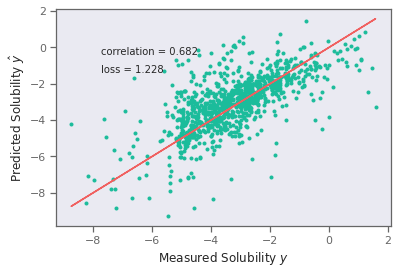
\includegraphics[width=0.8\linewidth]{fig/predict_solubility.png}
    \caption{เปรียบเทียบค่าสภาพการละลายที่ได้จากการทำนายและค่าอ้างอิง}
    \label{fig:pred_solubility}
\end{figure}

\end{enumerate}
